%=====================================================================
\section{Experimentación}

Esta sección cubre el entrenamiento (fase F6). Todo se hizo sobre las ventanas de validación 2023--2025; la prueba de 2026 no interviene.

\subsection{Registro de experimentos}

El registro de experimentos guarda, de cada entrenamiento, la etapa, el modelo, la configuración, la semilla, la ventana, el tamaño de entrenamiento, el AUC-PR y el AUC-ROC de validación, el tiempo y el número de parámetros. Hay \cifRegReferencias{} corridas de las referencias y \cifRegPropuesto{} del modelo propuesto:
\begin{itemize}
\item \cifRegBusq{} de la búsqueda;
\item \cifRegSens{} de la sensibilidad;
\item 15 de las semillas;
\item 3 de la variante sin evolución.
\end{itemize}
Los entrenamientos corren en paralelo (6 procesos). Uno del difuso-evolutivo con la configuración final tarda unos \cifTiempoFE{} minutos con unos 450\,000 commits, porque la aptitud se evalúa sobre una muestra de 80\,000.

\subsection{Búsqueda aleatoria}

Se evaluaron \cifNBusqueda{} configuraciones del espacio de la Tabla~\ref{tab:espacio} en las tres ventanas (Tabla~\ref{tab:busqueda}). La mejor tiene la población y el número de generaciones más grandes del espacio y la mutación más baja, y alcanza un AUC-PR medio de \cifMejorBusqueda{}. Que gane el extremo del espacio sugiere que el AG aún tenía margen. No se amplió la búsqueda: se registra como limitación.

\begin{table*}[!t]
\caption{Búsqueda aleatoria: AUC-PR medio $\pm$ desviación en las tres ventanas de validación (semilla 11)}
\label{tab:busqueda}
\centering\footnotesize
\begin{tabular}{@{}c c c c c c c c@{}}
\toprule
\cabecera \textbf{Puesto} & \textbf{Máx.\ reglas} & \textbf{Población} & \textbf{Generaciones} & \textbf{Prob.\ mutación} & \textbf{Prob.\ cruce} & $\boldsymbol{\lambda}$ & \textbf{AUC-PR}\\
\midrule
\filas{../comun/tabla_busqueda.tex}
\bottomrule
\end{tabular}
\end{table*}

\subsection{Análisis de sensibilidad}

Con el resto fijo en la mejor configuración, se varió el máximo de reglas y la probabilidad de mutación (Fig.~\ref{fig:sensibilidad}).

\textbf{La mutación es lo que más pesa.} Con 0,05 el AUC-PR medio es \cifSensMutBaja{}; con 0,30 baja a \cifSensMutAlta{}. Una mutación alta destruye las reglas buenas antes de que se propaguen.

\textbf{El máximo de reglas casi no importa.} El mejor punto (\cifSensMaxR{} reglas, mutación \cifSensMaxPm{}) da \cifSensMax{}, prácticamente igual que con 5 o 15. El peor es \cifSensMinR{} reglas con mutación \cifSensMinPm{}, con \cifSensMin{}. Esto es coherente con lo que el AG hace en la práctica: aunque se le permitan 15 reglas, termina usando entre \cifReglasMin{} y \cifReglasMax{}.

La configuración congelada es la de la búsqueda (15 reglas como máximo). No se cambió a 10 después de ver la sensibilidad, porque la diferencia (0,001) está dentro de la variación entre semillas.

\begin{figure}[!t]
\centering
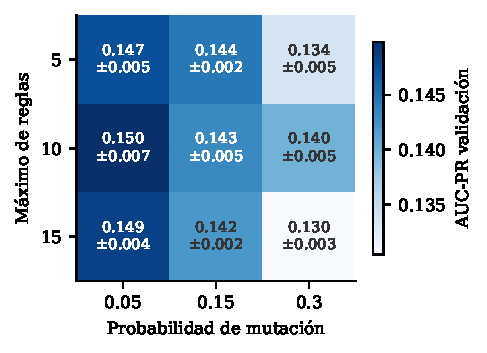
\includegraphics[width=0.82\columnwidth]{../../resultados/figuras/sensibilidad.pdf}
\caption{Sensibilidad: AUC-PR medio $\pm$ desviación en las tres ventanas, según el máximo de reglas y la probabilidad de mutación.}
\label{fig:sensibilidad}
\end{figure}

\subsection{Convergencia}

La Fig.~\ref{fig:convergencia} muestra la aptitud del mejor individuo y la mediana de la población, por generación, en la ventana 2025 para las 5 semillas. La mejora es rápida en las primeras 20 generaciones y se estabiliza entre la 60 y la 80. La distancia entre el mejor individuo y la mediana se mantiene, así que la población conserva diversidad hasta el final.

\begin{figure}[!t]
\centering
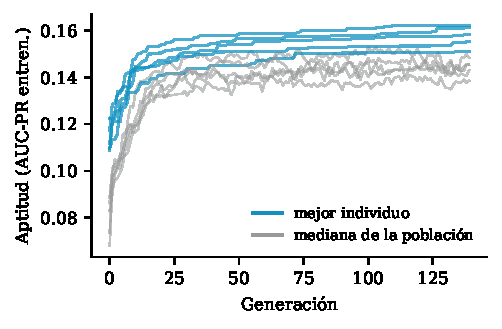
\includegraphics[width=0.92\columnwidth]{../../resultados/figuras/curva_aprendizaje.pdf}
\caption{Curva de aprendizaje del AG (ventana 2025, 5 semillas): aptitud del mejor individuo y mediana de la población.}
\label{fig:convergencia}
\end{figure}

\subsection{Semillas y aporte de la evolución}

La configuración elegida se entrenó con las 5 semillas (Tabla~\ref{tab:semillas}). El AUC-PR medio de validación es \cifValFE{} $\pm$ \cifValFEde{}. Es la diferencia observada respecto a las referencias, sin prueba de significancia todavía:
\begin{itemize}
\item prácticamente igual a la regresión logística (\cifValLogistica{});
\item el \cifRazonValFE{} del \emph{gradient boosting} (\cifValGB{});
\item muy por encima de la prevalencia.
\end{itemize}

La variante sin evolución arranca de la misma solución voraz y se queda en \cifValVariante{}. Usa \cifReglasVariante{} reglas con \cifAntVariante{} antecedentes. El AG no solo mejora el AUC-PR: también simplifica el modelo a entre \cifReglasMin{} y \cifReglasMax{} reglas, con \cifAntMin{} a \cifAntMax{} antecedentes en total.

\begin{table*}[!t]
\caption{Difuso-evolutivo con 5 semillas y variante sin evolución (validación)}
\label{tab:semillas}
\centering\footnotesize
\begin{tabular}{@{}l c c c c c c c@{}}
\toprule
\cabecera \textbf{Semilla} & \textbf{2023} & \textbf{2024} & \textbf{2025} & \textbf{Media} & \textbf{Reglas} & \textbf{Antec.} & \textbf{Tiempo (s)}\\
\midrule
\filas{../comun/tabla_semillas.tex}
\bottomrule
\end{tabular}
\end{table*}

\subsection{Configuración congelada}

Se congeló la configuración final antes de evaluar la prueba. Contiene:
\begin{itemize}
\item los hiperparámetros del difuso-evolutivo y las 5 semillas;
\item el umbral de MCC de cada semilla en la ventana 2025;
\item la semilla de referencia para McNemar (\cifSemillaRef{}, la de AUC-PR mediano);
\item la configuración y el umbral de cada referencia, con $R$ = \emph{gradient boosting};
\item la huella SHA-256 de la partición de prueba (\texttt{\cifHuella}\ldots).
\end{itemize}
El modelo final se entrena con todo 2019 hasta el 3 de octubre de 2025 y se evalúa una sola vez en 2026.
